\section{Theorie}
\label{sec:Theorie}
Ziel des Versuches ist die Bestimmung der effektiven Massen der Leitungselektronen in n-dotiertem Galiumarsenid.
Dazu wird der Faraday-Effekt verwendet. Dieser beschreibt die Drehung der Polarisationsebene eines Lichtstrahls, wenn dieser parallel zu einem Magnetfeld
ein transparentes Medium durchläuft.

\subsection{Bändermodell}
In einem Festkörper sind
Atomelektronen aus den inneren Schalen so stark an ihre Atome gebunden, dass sie wie bei freien Atomen nah um den Atomkern lokalisiert sind
und somit nicht wesentlich von den anderen Atomen beeinflusst werden. Deshalb werden nur die Elektronen in den äußeren Schalen betrachtet,
die durch die Wechselwirkung mit den Nachbarn delokalisiert sind und deshalb durch Blochwellen beschrieben werden können.
Die delokalisierten Elektronen befinden sich in Energiebändern, welche spezifisch für den jeweiligen Festkörper sind.
Wesentlich für Leitfähigkeit und andere Eigenschaften sind Valenz-und Leitungsband. Das Valenzband ist das letzte vollständig gefüllte Band.
Das Leitungsband ist das erste ungefüllte Band. Falls Elektronen in dieses angeregt werden, werden diese zu freien Ladungsträgern und tragen zur Leitfähigkeit bei.
Liegt zwischen Valenz-und Leitungsband eine Bandlücke (verbotener Bereich) $\Delta E_g >> k_B T$, so können auch bei höheren Temperaturen keine
Elektronen aus dem voll besetzten Band in das Leitungsband gelangen. Über den Wert der Bandlücke kann zwischen Leiter, Halbleiter und Nichtleiter
unterschieden werden \ref{pic:bander}. Leiter haben keine Bandlücke zwischen Valenz-und Leitungsband, während Nichtleiter eine Bandlücke von $\Delta E_g > \SI{5}{\eV}$ haben.
Halbleiter bewegen sich dazwischen und können durch thermische oder anderweitige Anregung Leitend werden. Bei Raumtemperatur ca. $T = 300 \si{\kelvin}$ fangen einige Halbleiter schon an zu leiten.
Jedoch benötigen die meisten Halbleiter deutlich höhere Temperaturen. Mithilfe der Boltzmann-Verteilung kann bei gegebener Temperatur die Anzahl der Ladungsträger im Valenzband bestimmt werden.
\begin{figure}
    \centering
    \includegraphics[width = 0.78\textwidth]{pics/Bänder.png}
    \caption{Unterscheidung nach Bandlücke.\cite{wikipedia}}
    \label{pic:bander}
\end{figure}

\subsection{Dotierung von Halbleitern}
In einen reinen Halbleiter können Fremdatome eingebaut werden um dessen elektronische Eigenschaften zu stark verändern.
Dabei wird zwischen einbringen von Donatoren (n-Dotierung) und Akzeptoren (p-Dotierung) unterschieden.
Bei der n-Dotierung werden Fremdatome mit einem zusätzlichen Valenzelektron eingebaut. Das zusätzliche Elektron ist über viele Gitteratome delokalisiert
und kann deshalb als frei angesehen werden. Es genügt also eine geringe Energie um das Elektron aus dem Donatorniveau in das Leitungsband anzuheben. 
Im Bänderschema des dotierten Halbleiters liegt das Donatorniveau somit dicht unter der Leitungsbandkante.
\begin{figure}
    \centering
    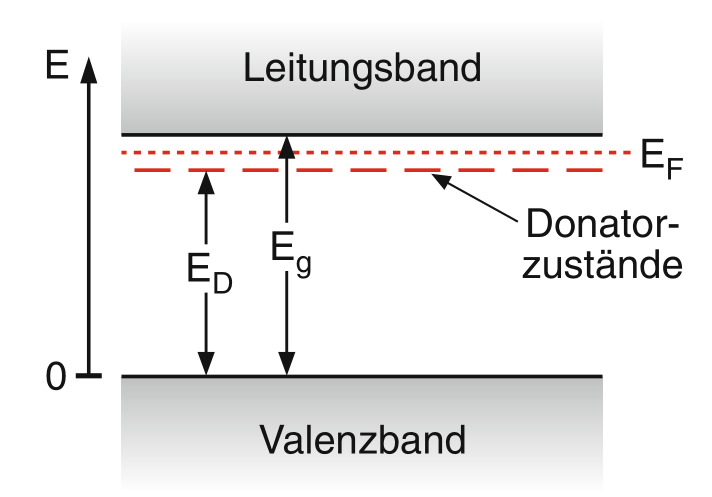
\includegraphics[width = 0.78\textwidth]{pics/n_dotierung.png}
    \caption{Bändermodell mit Donatorniveau.\cite{Demtröder3}}
    \label{pic:ndotierung}
\end{figure}
Bei einer p-Dotierung hingegen wird ein Fremdatom mit einem Valenzelektron weniger eingebaut. Es entsteht somit ein Akzeptatorniveau dicht oberhalb
des Valenzbands.

\subsection{Die effektive Masse}
Für freie Elektronen gilt die Dispersionsrelation
\begin{equation}
    E(\vec{k}) = \frac{\hbar^2 k^2}{2 m_e}
    \label{eqn:frei}
\end{equation}
mit der Energie E und der Wellenzahl k des Elektrons. Elektronen in einem Kristall verhalten sich als wären sie freie Teilchen. Jedoch mit einer veränderten Masse,
der sogenannten effektiven Masse $m*$. In quadratischer Näherung lässt sich die effektive Masse mit
\begin{equation}
    m^* = \hbar^2 \left(\frac{d^2 E}{d k_i d k_j}\right)^{-1}
\end{equation}
berechnen. 
 
\subsection{Zirkulare Doppelbrechung und Faraday-Effekt}
Eine linear polarisierte Welle kann als Überlagerung einer rechts und einer links zirkularen Welle dargestellt werden. Trifft diese nun auf ein
optisch aktives Medium kommt es zu einer Drehung der Polarisationsebene der Welle. Dieses Phänomen heißt zirkulare Doppelbrechung. 
In dem aktiven Medium wird die Phasengeschwindigkeit einer Drehrichtung erhöht und so ist beim Austreten die Polarisationsebene gedreht.
Die Polarisationsrichtung ändert sich proportional mit der zuückgelegten Strecke im Medium (der Dicke des Mediums).

Durch den Faraday Effekt können durchsichtige isotrope Substanzen optisch aktiv werden. Dazu wird ein Magnetfeld benötigt, welches parallel zur
Strahlrichtung ist. Der Drehwinkel lässt sich berechnen über
\begin{equation}
    \alpha = VBd
\end{equation}
mit der für den Stoff charakteristischen Größe V (Vernet-Konstante), der magnetischen Flussdichte $B$ und der Materialdicke $d$.
Die Richtung der Faraday-Drehung hängt dabei von der Richtung des Magnetfelds ab.
Mikroskopisch werden durch das Magnetfeld die freien Ladungsträger auf Kreisbahnen gezwungen. Die Rotation der Ladungsträger
führt dann zu einer bevorzugten Umlaufrichtung der zirkular polarisierten EM-Wellen und so zu einer Rotation der Polarisationsebene.
Somit ist die Doppelbrechung des Faraday-Effekts 
auch abhängig von der Anzahl an freien Ladungsträgern $N$.
Für quasifreie Ladungsträger ergibt sich für die Faradayrotation pro Einheitslänge $\theta_{frei} = \frac{\theta}{L}$ die Näherung
\begin{equation}
    \theta_{frei} \approx \frac{e_0^3}{8 \pi^2 \varepsilon_0 c^3} \frac{\lambda^2}{(m^*)^2}\frac{N B}{n}
    \label{eqn:theta}
\end{equation}
mit der Elementarladung $e_0$, der Influenzkonstante $\varepsilon_0$, der effektiven Masse $m^*$, der Magnetfeldstärke B, dem Brechungsindex n und der Lichtwellenlänge $\lambda$.





